\documentclass[a4paper, 12pt]{article}
\usepackage[T1,T2A]{fontenc}
\usepackage[utf8x]{inputenc}
\usepackage{graphicx}
\usepackage[labelsep=period]{caption}
\graphicspath{{pictures/}}
\usepackage[english,russian]{babel}
\usepackage{amsmath}
\usepackage{color,graphicx,ulem,cmap}
\usepackage{subfigure}
\title{основная часть}
\author{я}
\begin{document}


\begin{figure}[ht!]  
\vspace{-4ex} \centering \subfigure[]{
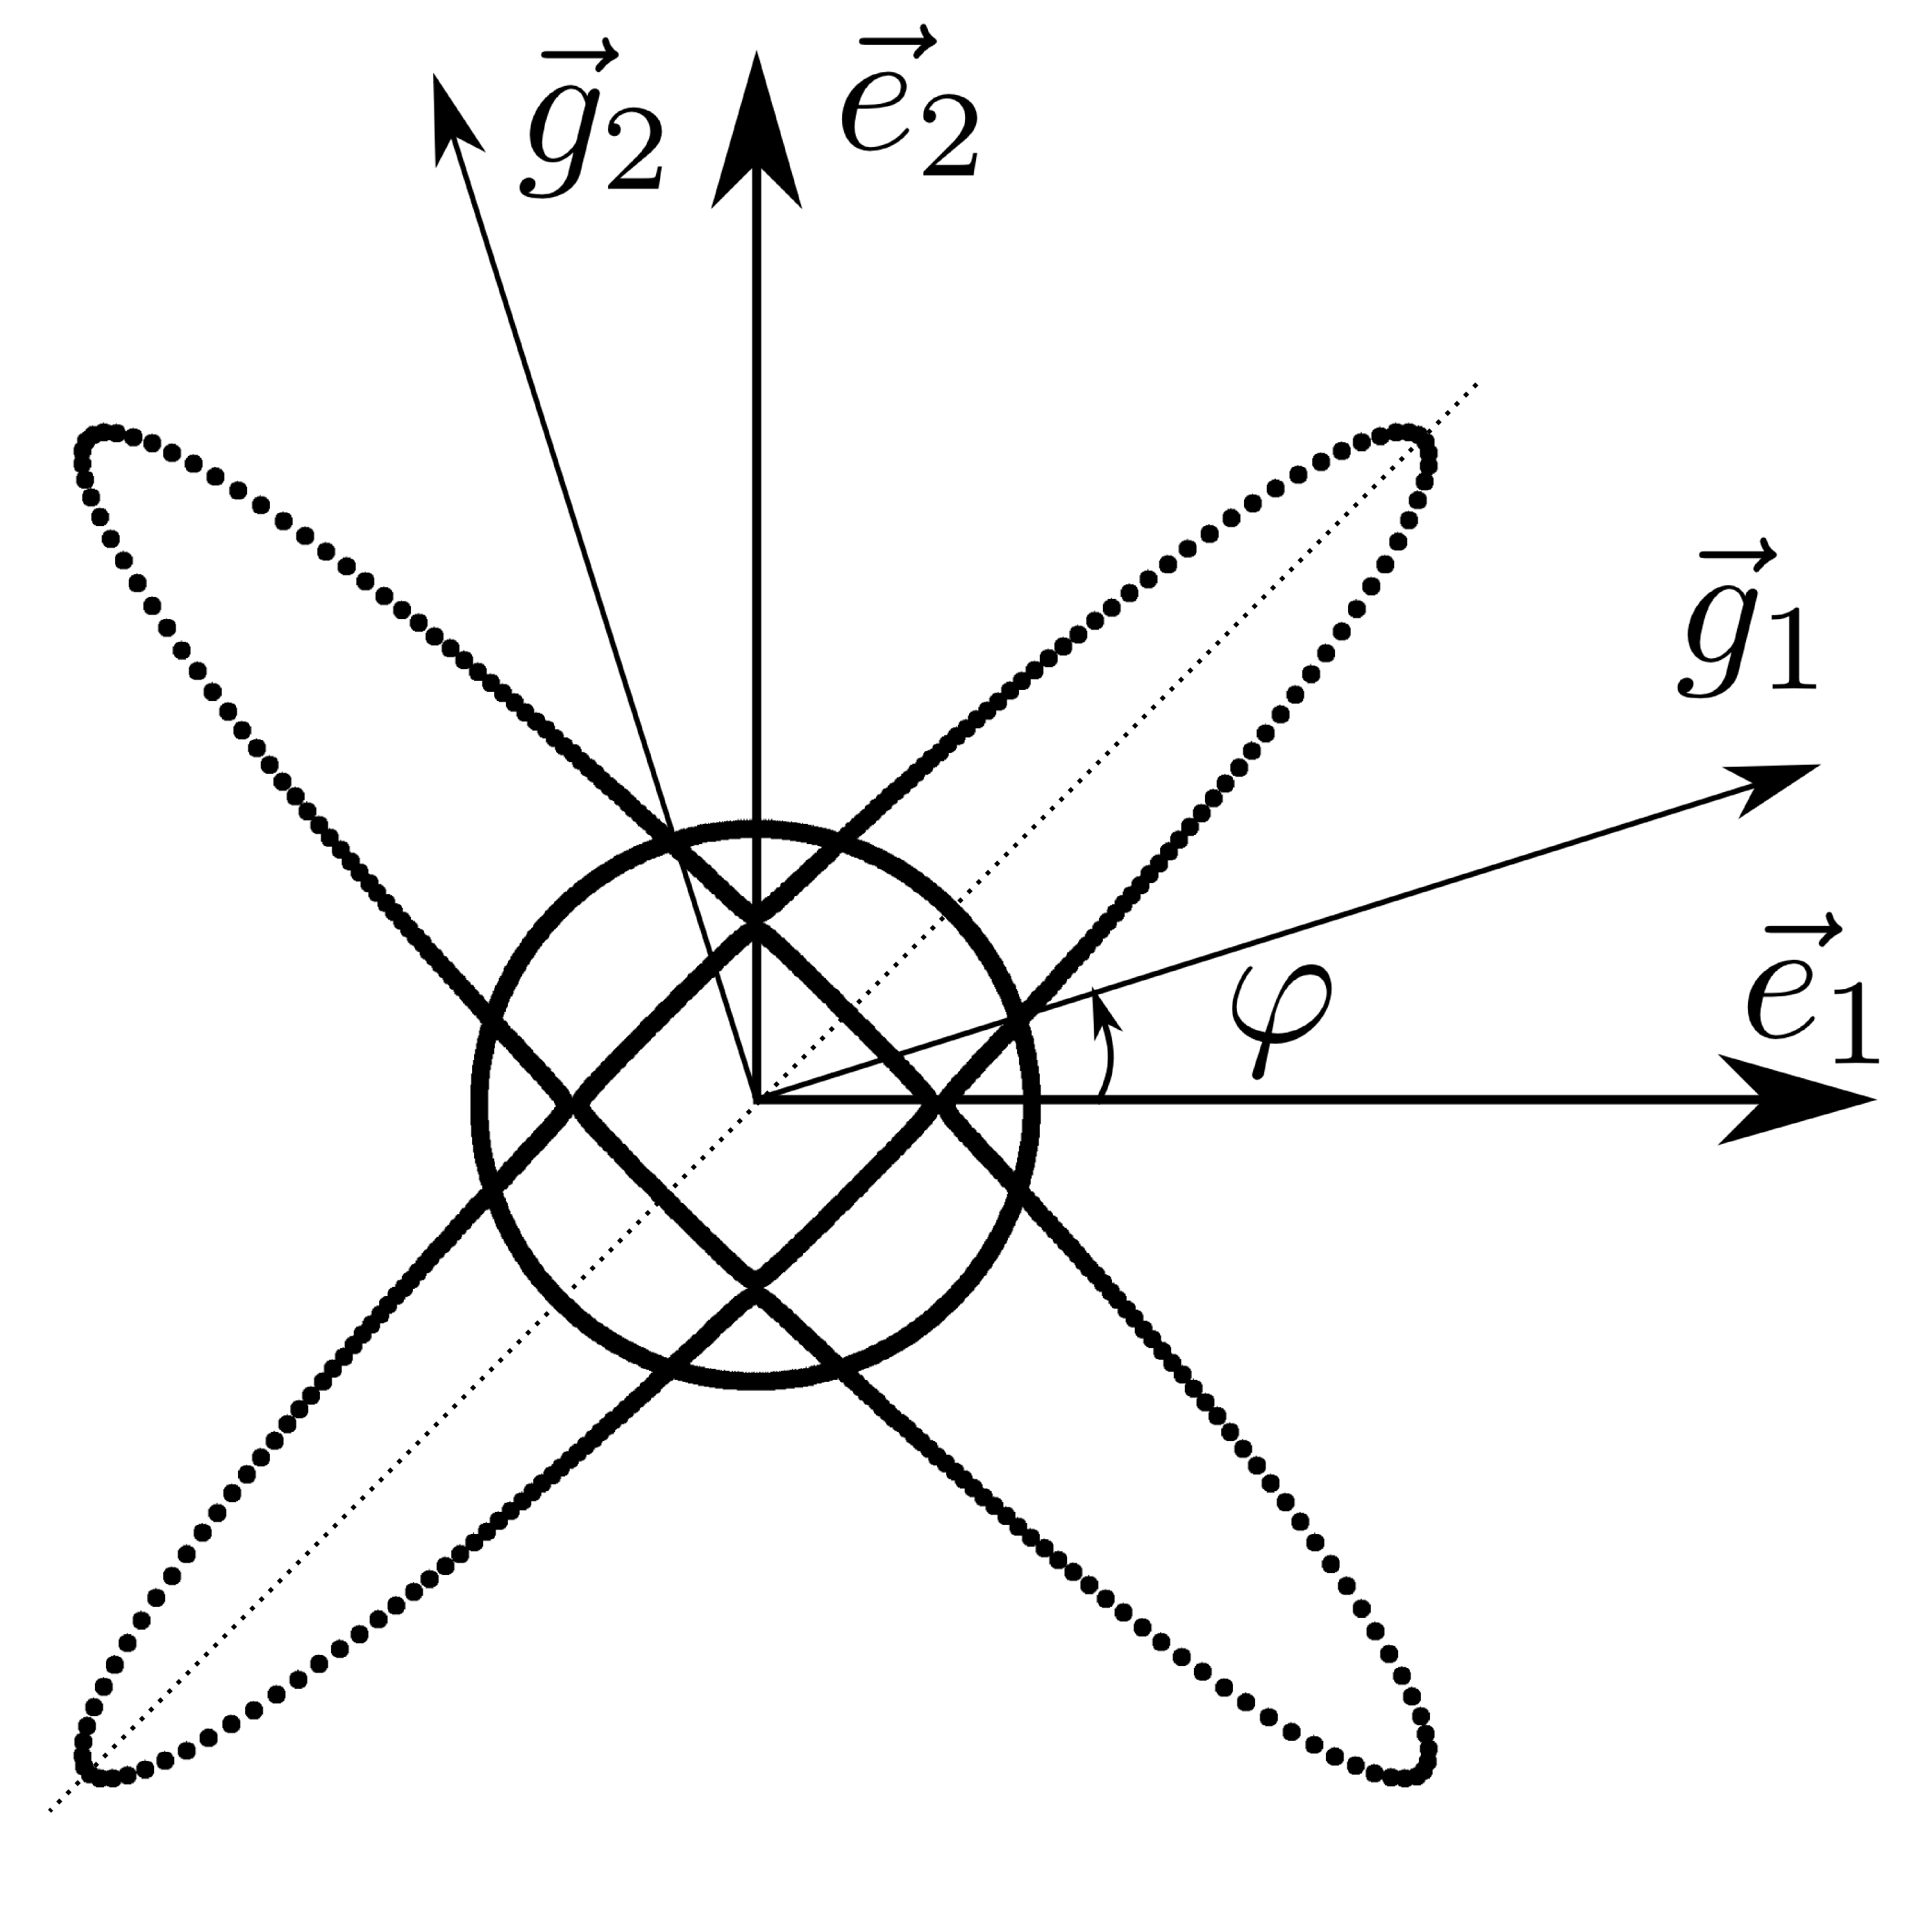
\includegraphics[width=0.40\linewidth]{teo2_xy_0_deg_rot_ax.png} \label{XY_axis_a} }  
\hspace{4ex}
\subfigure[]{
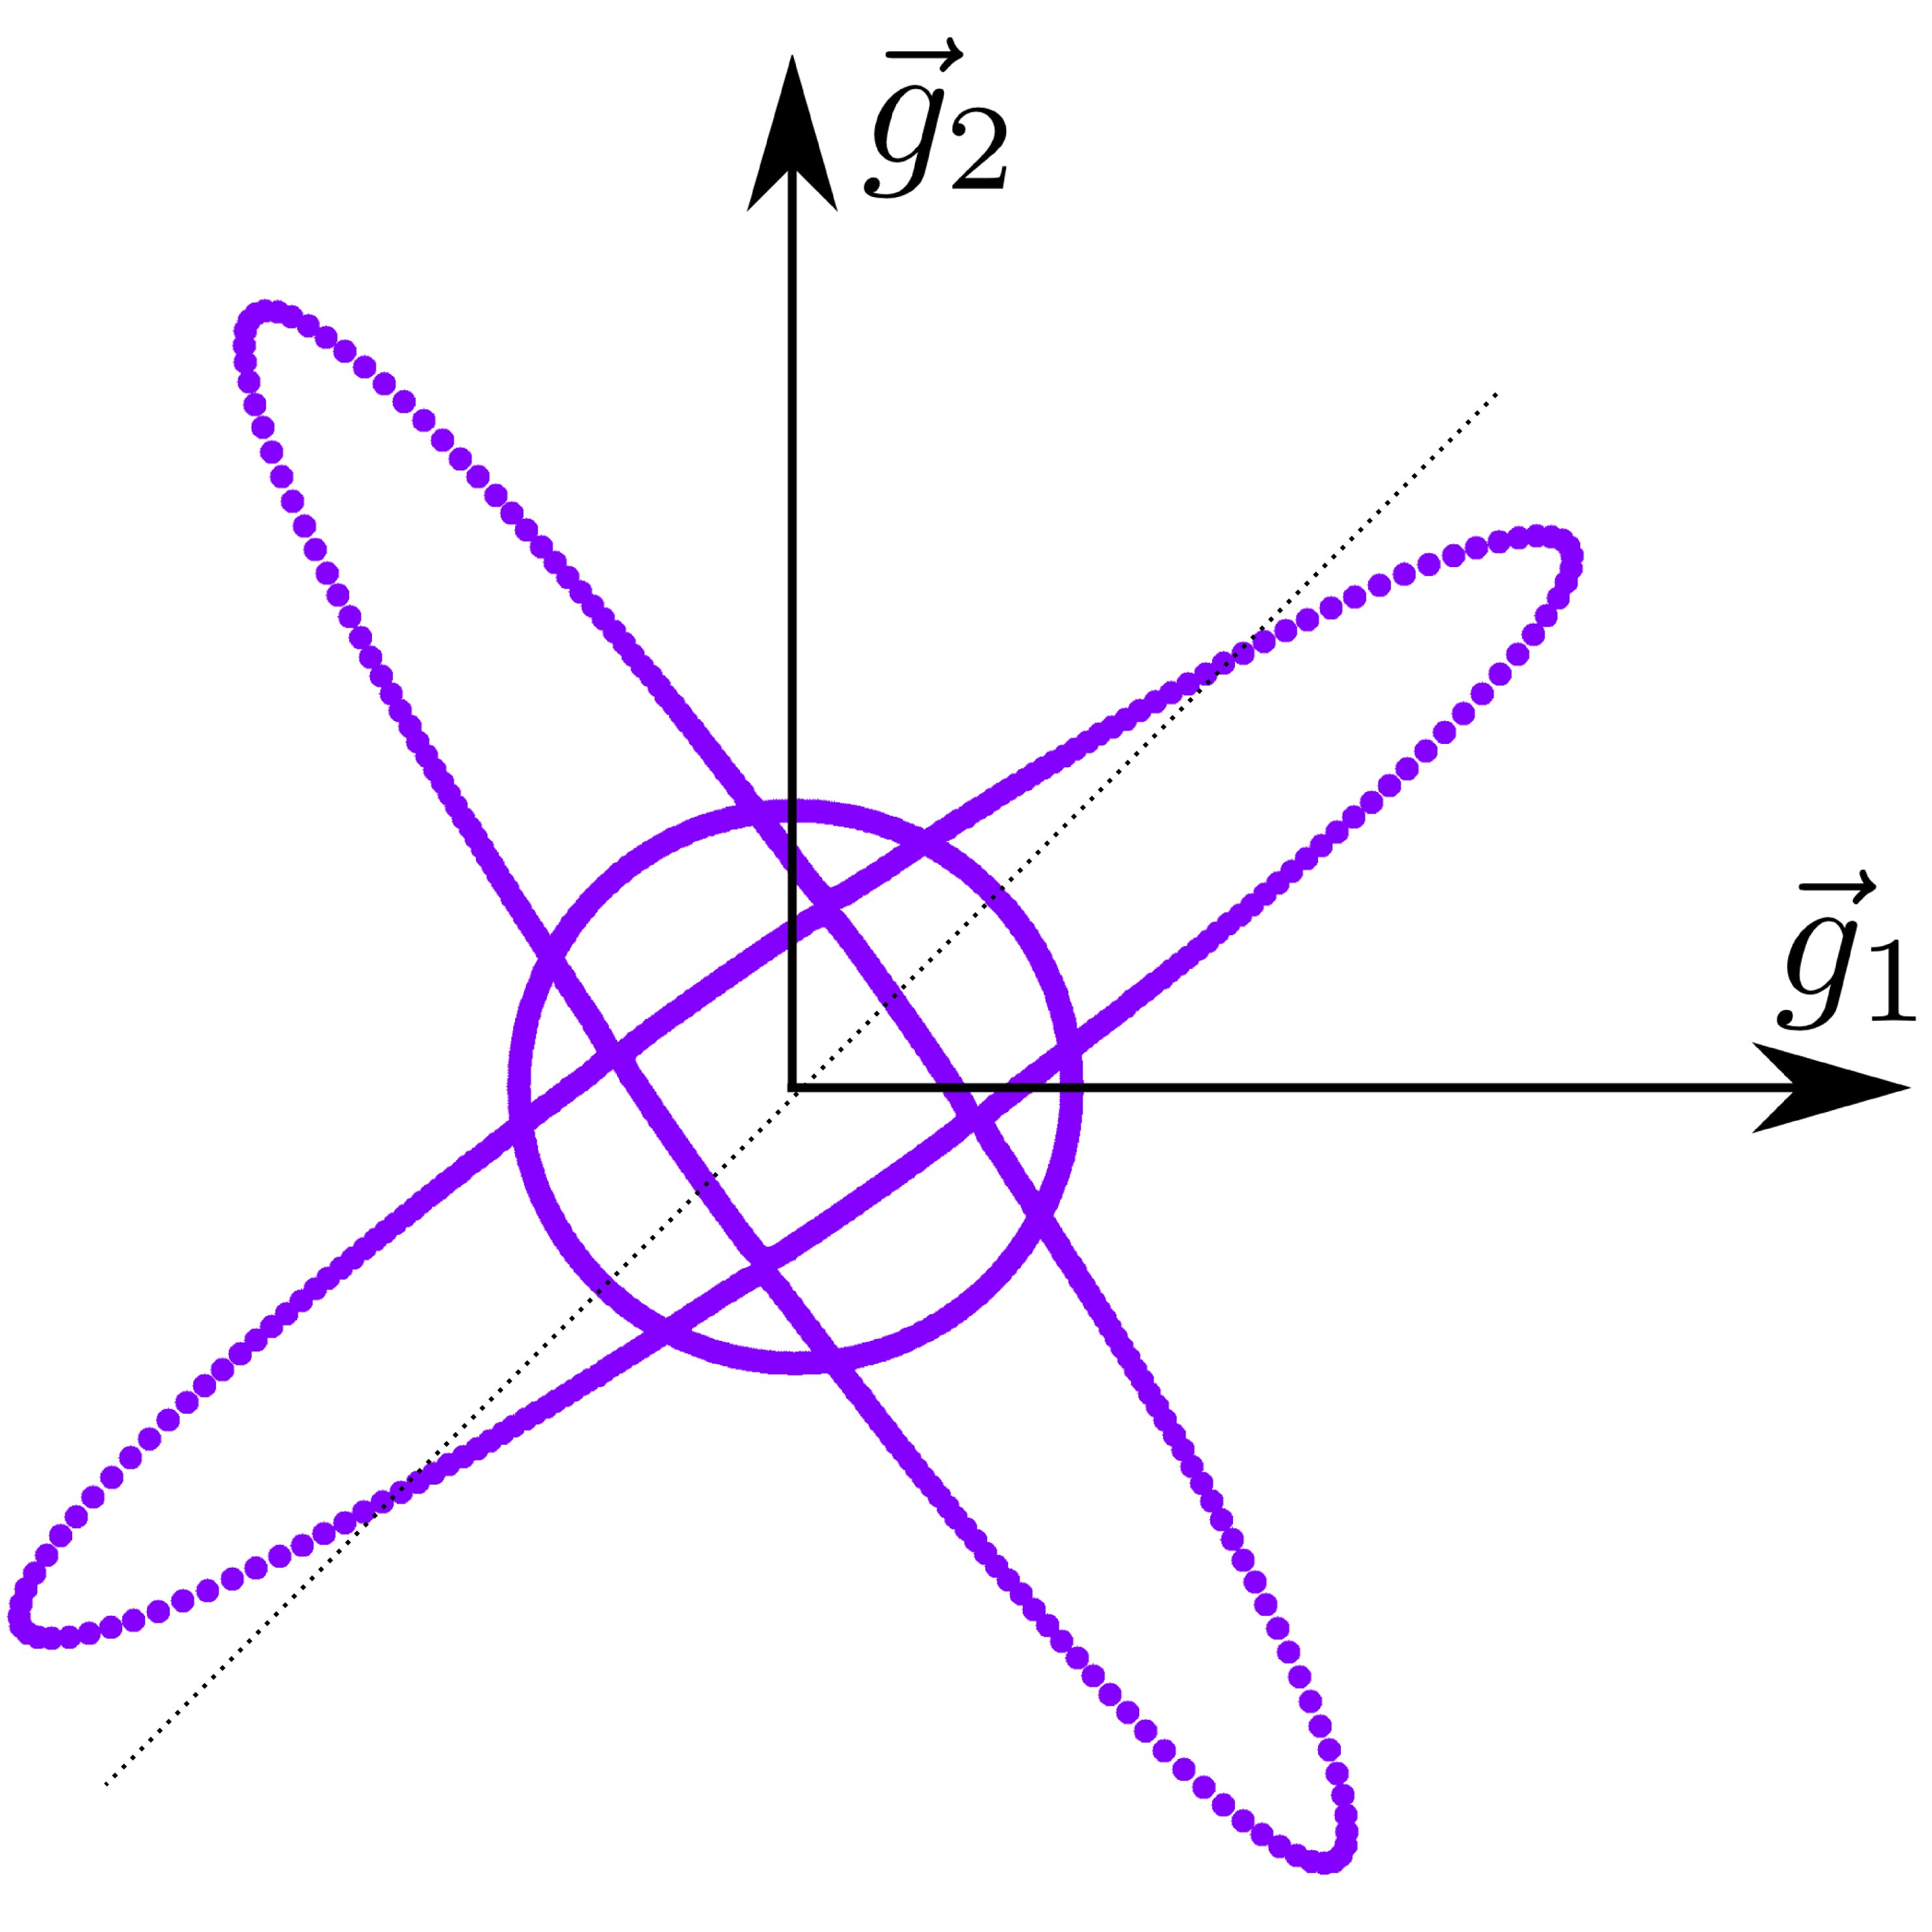
\includegraphics[width=0.40\linewidth]{teo2_xy_10_deg_rot_ax.png} \label{XY_axis_b} }
\hspace{4ex}  
\caption{Проекция поверхности медленности в различных координатный осях} \label{XY_axis}
\end{figure}

\end{document}
